\documentclass{article}


\ifdefined\EXERCISE
%\documentclass[11pt]{article}
\documentclass[11pt, twoside]{book}
\else
\documentclass[11pt, openright, twoside]{book}
\fi
\usepackage{libertine}
\newcommand{\bookflag}{ } 
%\usepackage{courier}
\usepackage[utf8]{inputenc}
\ifdefined \bookflag
  \usepackage[a4paper, marginparwidth=100pt, total={5in, 9in}]{geometry}
\else
\usepackage[a4paper, total={6in, 9in}]{geometry}
\fi
\usepackage{braket}
\usepackage{xcolor}
\usepackage{amsmath}
\usepackage{amsfonts}
\usepackage{amsthm}
\usepackage{amssymb}
%\usepackage[ocgcolorlinks]{hyperref}
\usepackage{titling}
\usepackage{hyperref}
%\usepackage{hyperref,xcolor}
%\usepackage[ocgcolorlinks]{ocgx2}
\usepackage{cleveref}
\usepackage{graphicx}
\usepackage{svg}
\usepackage{float}
\usepackage{wrapfig}
\usepackage{tikz}
\usetikzlibrary{patterns, shapes.arrows}
\usetikzlibrary{calc, positioning,fit,intersections}
\usetikzlibrary{arrows.meta,bending}
\usetikzlibrary{decorations.pathreplacing,angles,quotes}
\usetikzlibrary{animations}
\usepackage{adjustbox}
%\usepackage{tikz-network}
\usepackage{tkz-graph}
\usetikzlibrary{decorations.pathmorphing}
\usepackage{tkz-berge}
\usepackage[linesnumbered]{algorithm2e}
\usepackage{multicol}
\usepackage[backend=biber,style=alphabetic,sorting=ynt]{biblatex}
%\usepackage{xcolor}
%\usepackage{tkz-berge}
%\usepackage{tkz-graph}
\usepackage{pgfplots}
\usepackage{setspace}
\usepackage{etoc}
%\usepackage{wrapfig}
\usepackage{pgfgantt}
\usepackage{pdfpages}
\DeclareUnicodeCharacter{2212}{−}
\usepgfplotslibrary{groupplots,dateplot}
\pgfplotsset{compat=newest}


\ifdefined\BOOK
\else
\usepackage{chngcntr}
\counterwithout{section}{chapter}

\fi
\newcommand{\mynewtheorem}[2]{  
  \newtheorem{#1}{#2}
  \ifdefined\BOOK
  \numberwithin{#1}{section}
  \fi

}
\newcommand{\mynewtheoremstar}[2]{  
  \newtheorem*{#1}{#2}

}

\theoremstyle{plain}
\mynewtheorem{theorem}{Theorem}
\mynewtheoremstar{theorem*}{Theorem}
\mynewtheorem{lemma}{Lemma}
\mynewtheorem{claim}{Claim}
\mynewtheorem{problem}{Problem}
\mynewtheorem{exercise}{Exercise}
\theoremstyle{definition}
\mynewtheorem{definition}{Definition}
\theoremstyle{remark}
\mynewtheorem{corollary}{Corollary}
\mynewtheorem{example}{Example}
\mynewtheorem{fact}{Fact}
\mynewtheorem{remark}{Remark}
\mynewtheorem{conjecture}{Conjecture}
\mynewtheorem{solution}{Solution}
\mynewtheorem{openproblem}{Open problem}
\crefname{lemma}{Lemma}{Lemmas}
\Crefname{algocf}{Algorithm}{Algorithms}
\hypersetup{colorlinks=true}
% , allcolors=blue,allbordercolors=blue,pdfborderstyle={0 0 1}}
%\hypersetup{pdfborder={2 2 2}}
% pdfpagemode=FullScreen,
% backref 

\crefname{problem}{Problem}{Problems}

\DeclareMathOperator{\Ima}{Im}
\DeclareMathOperator{\Rea}{Re}
\DeclareMathOperator{\rank}{rank}
\DeclareMathOperator{\sign}{sign}


\usepackage{adjustbox}
\usepackage{subcaption}
\usetikzlibrary{calc}
\usepackage{array}
%\usepackage[vlined,linesnumbered]{algorithm2e}
\usepackage[bottom]{footmisc}

\usepackage[
backend=biber,
style=alphabetic,
sorting=ynt
]{biblatex}

\usepackage{tcolorbox}
\usepackage{marginnote}
 
%https://osl.ugr.es/CTAN/macros/latex/contrib/tcolorbox/tcolorbox.pdf
\tcbuselibrary{breakable}
\tcbset{%any default parameters
  width=0.9\textwidth,
  halign=justify,
  center,
  breakable,
  colback=white    
}
\newtcolorbox{algbox}[1]{colback=blue!5!white,
colframe=blue!75!black,fonttitle=\bfseries,
title={#1},float=f}
\newtcolorbox{defbox}[1]{colback=blue!5!white,
colframe=red!75!black,fonttitle=\bfseries,
title={#1}}

\SetKwProg{Fn}{Function}{}{end}


\newcommand{\commentt}[1]{\textcolor{blue}{ \textbf{[COMMENT]} #1}}
\newcommand{\ctt}[1]{\commentt{#1}}
\newcommand{\prb}[1]{ \mathbf{Pr} \left[ {#1} \right]}
\newcommand{\onotation}[1]{\(\mathcal{O} \left( {#1}  \right) \)}
\newcommand{\ona}[1]{\onotation{#1}}
\newcommand{\nvar}[2]{ \( #1_{1}, #1_{2} ... #1_{#2}  \) }

% \addbibresource{sample.bib} %Import the bibliography file
\begin{document}    
\maketitle

% Supplementary material: a geometric view of the Master Theorem.
% Source and interactive version: https://elyg121.github.io/visualizing-the-master-theorem/

\usetikzlibrary{decorations.pathreplacing}

\definecolor{primary}{RGB}{37, 99, 235}
\definecolor{secondary}{RGB}{71, 85, 105}
\definecolor{accent1}{RGB}{16, 185, 129} % Green for leaves
\definecolor{accent2}{RGB}{239, 68, 68}  % Red for root
\definecolor{accent3}{RGB}{245, 158, 11} % Amber for balanced

\newtcolorbox{educatortip}[1][Educator Tip]{
    colback=primary!5,
    colframe=primary,
    title=\textbf{#1}
}

\begin{document}
\ifdefined\BOOK
  \chapter{The Geometry of the Master Theorem}
\else
  \chapter*{The Geometry of the Master Theorem}
\fi

\noindent\textit{A Visual Guide to Divide and Conquer} \hfill Ely Grunfeld

\begin{tcolorbox}[colback=primary!5, colframe=primary, title=\textbf{Supplementary Material (Educator Version)}]
This guide supplements the recitation on the Master Theorem. An interactive version, in English and Hebrew, with student and educator modes, is available at \href{https://elyg121.github.io/visualizing-the-master-theorem/}{\nolinkurl{elyg121.github.io/visualizing-the-master-theorem}}.
\end{tcolorbox}
\section{Introduction}

The goal of this document is to provide educators with a highly intuitive, visually memorable framework for teaching the Master Theorem. 

The initial sections, ``The Divide and Conquer Strategy'' and ``Building the Recursion Tree,'' establish the foundational intuition behind the recursive formula and its tree-graph representation. While standard derivations of these concepts exist across many resources, they are included here to lay the necessary groundwork. 

The core novelty of this guide lies in the final section: \textbf{translating the three cases of the Master Theorem into three distinct geometric shapes}—a triangle, a rectangle, and an inverted triangle.

\section{The Divide and Conquer Strategy}

The Master Theorem is a tool used to analyze the runtime of algorithms that employ a \textbf{divide and conquer} strategy. Instead of solving a massive problem all at once, these algorithms do three things:
\begin{enumerate}
    \item \textbf{Divide:} Break the large problem into several smaller, identical subproblems.
    \item \textbf{Conquer:} Solve those smaller subproblems recursively.
    \item \textbf{Combine:} Glue the solutions of the subproblems back together to form the final answer.
\end{enumerate}
% TODO add merge sort and binary search examples
To make this concrete, let's look at two classic examples of divide and conquer algorithms. \textbf{Merge Sort} recursively splits an array into two halves until each element is isolated, and then merges those sorted sub-arrays back together to form the final sorted output. \textbf{Binary Search} locates a target value in a sorted array by repeatedly dividing the search interval in half and recursively exploring only the side where the target could exist.

\begin{figure}[htpb!]
    \centering
    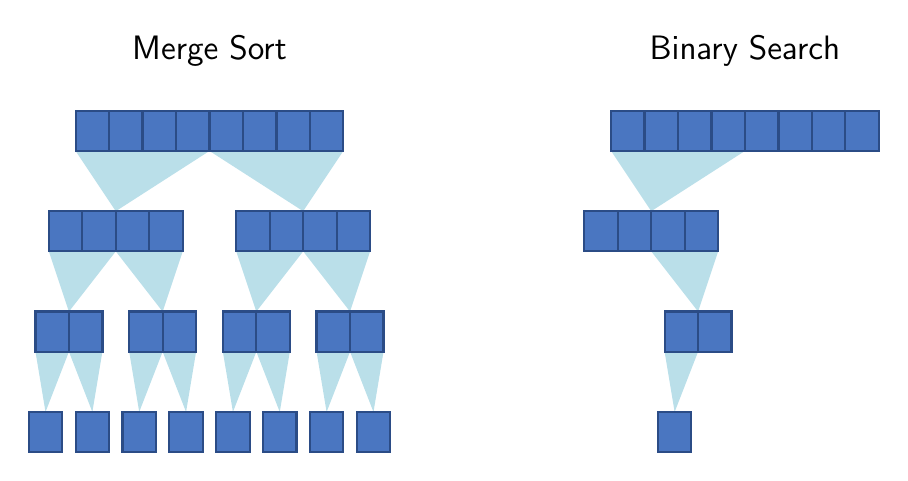
\begin{tikzpicture}[scale=0.85, transform shape]
        % Define Case 2 (Rectangle) colors
        \definecolor{case2blue}{RGB}{74,118,193}
        \definecolor{case2light}{RGB}{186,223,233}
        \definecolor{case2border}{RGB}{43,76,134}

        % --- MERGE SORT ---
        \node at (-2.0, 6.0) {\Large \sffamily Merge Sort};

        % Triangles Layer 1 -> Layer 2
        \fill[case2light] (-4.0, 4.5) -- (-2.0, 4.5) -- (-3.4, 3.6) -- cycle;
        \fill[case2light] (-2.0, 4.5) -- (0.0, 4.5) -- (-0.6, 3.6) -- cycle;

        % Triangles Layer 2 -> Layer 3
        \fill[case2light] (-4.4, 3.0) -- (-3.4, 3.0) -- (-4.1, 2.1) -- cycle;
        \fill[case2light] (-3.4, 3.0) -- (-2.4, 3.0) -- (-2.7, 2.1) -- cycle;
        \fill[case2light] (-1.6, 3.0) -- (-0.6, 3.0) -- (-1.3, 2.1) -- cycle;
        \fill[case2light] (-0.6, 3.0) -- (0.4, 3.0) -- (0.1, 2.1) -- cycle;

        % Triangles Layer 3 -> Layer 4
        \fill[case2light] (-4.6, 1.5) -- (-4.1, 1.5) -- (-4.45, 0.6) -- cycle;
        \fill[case2light] (-4.1, 1.5) -- (-3.6, 1.5) -- (-3.75, 0.6) -- cycle;
        \fill[case2light] (-3.2, 1.5) -- (-2.7, 1.5) -- (-3.05, 0.6) -- cycle;
        \fill[case2light] (-2.7, 1.5) -- (-2.2, 1.5) -- (-2.35, 0.6) -- cycle;
        \fill[case2light] (-1.8, 1.5) -- (-1.3, 1.5) -- (-1.65, 0.6) -- cycle;
        \fill[case2light] (-1.3, 1.5) -- (-0.8, 1.5) -- (-0.95, 0.6) -- cycle;
        \fill[case2light] (-0.4, 1.5) -- (0.1, 1.5) -- (-0.25, 0.6) -- cycle;
        \fill[case2light] (0.1, 1.5) -- (0.6, 1.5) -- (0.45, 0.6) -- cycle;

        % Boxes Layer 1 (Size 8 array)
        \foreach \x in {-4.0, -3.5, -3.0, -2.5, -2.0, -1.5, -1.0, -0.5} {
            \draw[thick, case2border, fill=case2blue] (\x, 4.5) rectangle (\x+0.5, 5.1);
        }

        % Boxes Layer 2 (Two Size 4 arrays)
        \foreach \x in {-4.4, -3.9, -3.4, -2.9, -1.6, -1.1, -0.6, -0.1} {
            \draw[thick, case2border, fill=case2blue] (\x, 3.0) rectangle (\x+0.5, 3.6);
        }

        % Boxes Layer 3 (Four Size 2 arrays)
        \foreach \x in {-4.6, -4.1, -3.2, -2.7, -1.8, -1.3, -0.4, 0.1} {
            \draw[thick, case2border, fill=case2blue] (\x, 1.5) rectangle (\x+0.5, 2.1);
        }

        % Boxes Layer 4 (Eight Size 1 arrays)
        \foreach \x in {-4.7, -4.0, -3.3, -2.6, -1.9, -1.2, -0.5, 0.2} {
            \draw[thick, case2border, fill=case2blue] (\x, 0.0) rectangle (\x+0.5, 0.6);
        }


        % --- BINARY SEARCH ---
        \node at (6.0, 6.0) {\Large \sffamily Binary Search};

        % Triangle L1 -> L2 (Picking the Left Half)
        \fill[case2light] (4.0, 4.5) -- (6.0, 4.5) -- (4.6, 3.6) -- cycle;
        
        % Triangle L2 -> L3 (Picking the Right Half)
        \fill[case2light] (4.6, 3.0) -- (5.6, 3.0) -- (5.3, 2.1) -- cycle;

        % Triangle L3 -> L4 (Picking the Left Half)
        \fill[case2light] (4.8, 1.5) -- (5.3, 1.5) -- (4.95, 0.6) -- cycle;

        % Boxes Layer 1 (Size 8 array)
        \foreach \x in {4.0, 4.5, 5.0, 5.5, 6.0, 6.5, 7.0, 7.5} {
            \draw[thick, case2border, fill=case2blue] (\x, 4.5) rectangle (\x+0.5, 5.1);
        }

        % Boxes Layer 2 (One Size 4 array)
        \foreach \x in {3.6, 4.1, 4.6, 5.1} {
            \draw[thick, case2border, fill=case2blue] (\x, 3.0) rectangle (\x+0.5, 3.6);
        }

        % Boxes Layer 3 (One Size 2 array)
        \foreach \x in {4.8, 5.3} {
            \draw[thick, case2border, fill=case2blue] (\x, 1.5) rectangle (\x+0.5, 2.1);
        }

        % Boxes Layer 4 (One Size 1 array)
        \foreach \x in {4.7} {
            \draw[thick, case2border, fill=case2blue] (\x, 0.0) rectangle (\x+0.5, 0.6);
        }

    \end{tikzpicture}
    \caption{Merge Sort branching out to process all subproblems compared to Binary Search following only a single subproblem path.}
\end{figure}
\subsection{Deriving the Formula}

The divide and conquer strategy is inherently recursive because the subproblems it generates are simply smaller instances of the original problem, allowing the algorithm to call itself to solve them. Consequently, we can derive a recursive formula to describe the runtime of these algorithms. We define the following elements:
\begin{itemize}
    \item $n$: The size of our initial problem.
    \item $T$: The total runtime function. For example, evaluating this function at input $n$, written as $T(n)$, gives the total time it takes to solve a problem of size $n$.
    \item $a$: The number of smaller subproblems we split our big problem into (where $a \ge 1$).
    \item $b$: The factor by which the problem size shrinks. For example, if we cut the problem in half, $b = 2$. This means each new subproblem has a size of $n/b$ (where $b > 1$).
    \item $f$: The ``overhead'' work function. For example, $f(n)$ represents the time required to physically divide a problem of size $n$ at the start, plus the time to combine all its subproblem answers at the end.
\end{itemize}
Mapping these variables to our examples:
\begin{itemize}
    \item Merge Sort divides the array in two ($b=2$), recurses on both halves ($a=2$), and merges in linear time ($f(n) = \Theta(n)$).

    \item  Binary Search also halves the array ($b=2$), but recurses on just one half ($a=1$) with constant overhead work ($f(n) = \Theta(1)$).
\end{itemize}


To establish the complete runtime $T(n)$, we define a base case and construct the general equation by adding its two core components:

\begin{itemize}
    \item Time spent on recursive work: Because each subproblem is exactly the same as the initial problem but reduced to a size of $\frac{n}{b}$, solving just one takes $T\left(\frac{n}{b}\right)$ time. Since the algorithm generates $a$ of these subproblems, we multiply to find the total recursive time: $aT\left(\frac{n}{b}\right)$.

    \item Overhead work: $f(n)$, which accounts for the time spent physically dividing the problem and combining the recursive answers. 

    \item Anchoring the recursive formula: To formally anchor this recursion, we assume a base case of $T(1) = \Theta(1)$ and $f(1) = \Theta(1)$. This simply means that when the problem size is reduced to a single element, the algorithm takes a constant amount of time to process it and no further division is required.
\end{itemize}

Setting the total time $T(n)$ equal to the recursive work plus the overhead work naturally builds our standard recurrence relation:
\[ T(n) = aT\left(\frac{n}{b}\right) + f(n) \quad \text{for } n > 1 \]
\[ T(1) = \Theta(1) \]

 To avoid using rounding functions like floor and ceiling, we will assume $n$ is an exact power of $b$. While this simplification keeps the math clean, the explanation and the Master Theorem hold true even when $n$ is not an exact power of $b$. Because our ultimate goal is to analyze asymptotic behavior, omitting these rounding functions does not alter the final complexity bounds.

Applying this general formula to our earlier examples yields their exact recurrence relations:
\begin{itemize}
    \item \textbf{Merge Sort:} $T(n) = 2T\left(\frac{n}{2}\right) + \Theta(n)$
    \item \textbf{Binary Search:} $T(n) = T\left(\frac{n}{2}\right) + \Theta(1)$
\end{itemize}

\begin{educatortip}
Ground the recursive formula by having students explicitly map abstract variables like $a$, $b$, and $f(n)$ to familiar algorithms on the board. This makes the mathematical components tangible.
\end{educatortip}

Our objective is to resolve this recurrence relation to find the asymptotic behavior of $T(n)$ directly in terms of $n$. To accomplish this, we can visualize the total work done by the algorithm using a \textbf{recursion tree}.

\section{Building the Recursion Tree}
When we unfold the recurrence relation, we create a tree structure where each node represents the cost of a single subproblem.
% TODO: add tree image
\begin{figure}[htpb!]
    \centering
    \begin{adjustbox}{max width=\linewidth}
    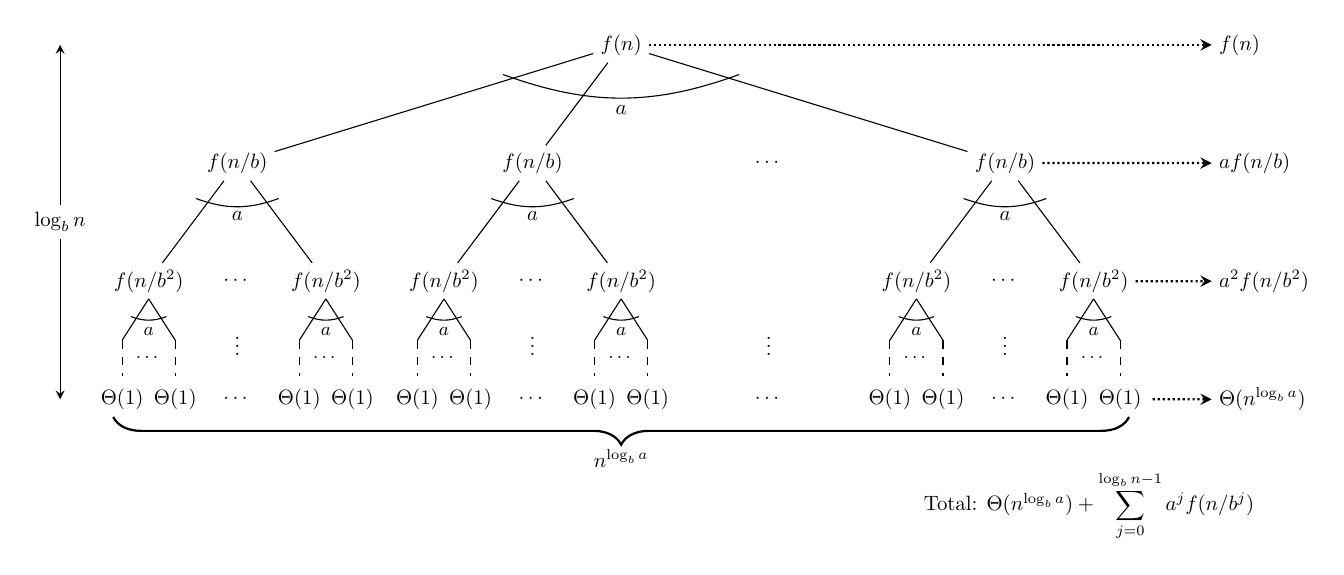
\begin{tikzpicture}[scale=0.75, transform shape]
        
        % Root Node
        \node (root) at (0,0) {$f(n)$};
        
        % Level 1 Nodes - Spread out horizontally to prevent overlap
        \node (L1a) at (-6.5,-2) {$f(n/b)$};
        \node (L1b) at (-1.5,-2) {$f(n/b)$};
        \node (L1c) at (2.5,-2) {$\cdots$};
        \node (L1d) at (6.5,-2) {$f(n/b)$};
        
        \draw (root) -- (L1a);
        \draw (root) -- (L1b);
        \draw (root) -- (L1d);
        
        % Arc for 'a' branches at root
        \draw (-2,-0.5) to[bend right=20] (2,-0.5);
        \node at (0,-1.1) {$a$};
        
        % Level 2 for L1a
        \node (L2a1) at (-8,-4) {$f(n/b^2)$};
        \node (L2a2) at (-6.5,-4) {$\cdots$};
        \node (L2a3) at (-5,-4) {$f(n/b^2)$};
        \draw (L1a) -- (L2a1);
        \draw (L1a) -- (L2a3);
        \draw (-7.2,-2.6) to[bend right=20] (-5.8,-2.6);
        \node at (-6.5,-2.9) {$a$};

        % Level 2 for L1b
        \node (L2b1) at (-3,-4) {$f(n/b^2)$};
        \node (L2b2) at (-1.5,-4) {$\cdots$};
        \node (L2b3) at (0,-4) {$f(n/b^2)$};
        \draw (L1b) -- (L2b1);
        \draw (L1b) -- (L2b3);
        \draw (-2.2,-2.6) to[bend right=20] (-0.8,-2.6);
        \node at (-1.5,-2.9) {$a$};
        
        % Level 2 for L1d
        \node (L2d1) at (5,-4) {$f(n/b^2)$};
        \node (L2d2) at (6.5,-4) {$\cdots$};
        \node (L2d3) at (8,-4) {$f(n/b^2)$};
        \draw (L1d) -- (L2d1);
        \draw (L1d) -- (L2d3);
        \draw (5.8,-2.6) to[bend right=20] (7.2,-2.6);
        \node at (6.5,-2.9) {$a$};

        % Vertical Dots continuing downward
        \node at (-6.5,-5) {$\vdots$};
        \node at (-1.5,-5) {$\vdots$};
        \node at (2.5,-5) {$\vdots$};
        \node at (6.5,-5) {$\vdots$};
        
        % Leaf Nodes \cdots for the gaps
        \node at (-6.5,-6) {$\cdots$};
        \node at (-1.5,-6) {$\cdots$};
        \node at (2.5,-6) {$\cdots$};
        \node at (6.5,-6) {$\cdots$};

        % Level 3 Branches and Theta(1) Leaves
        \foreach \x in {-8, -5, -3, 0, 5, 8} {
            % Solid branch lines (narrowed slightly to completely eliminate overlap)
            \draw (\x, -4.3) -- (\x-0.45, -5.0);
            \draw (\x, -4.3) -- (\x+0.45, -5.0);
            
            % Arc and 'a' label
            \draw (\x-0.3, -4.6) to[bend right=20] (\x+0.3, -4.6);
            \node at (\x, -4.85) {\small $a$};
            
            % Dashed continuation
            \draw[dashed, thin] (\x-0.45, -5.0) -- (\x-0.45, -5.6);
            \draw[dashed, thin] (\x+0.45, -5.0) -- (\x+0.45, -5.6);
            
            % Dots between dashed lines
            \node at (\x, -5.3) {\small $\dots$};
            
            % Theta(1) leaves properly aligned to branches
            \node at (\x-0.45, -6) {$\Theta(1)$};
            \node at (\x+0.45, -6) {$\Theta(1)$};
        }

        % Row Sums on the right side
        \node[anchor=west] (sum0) at (10,0) {$f(n)$};
        \node[anchor=west] (sum1) at (10,-2) {$a f(n/b)$};
        \node[anchor=west] (sum2) at (10,-4) {$a^2 f(n/b^2)$};
        \node[anchor=west] (sum3) at (10,-6) {$\Theta(n^{\log_b a})$};
        
        \draw[densely dotted, thick, -stealth] (root) -- (sum0);
        \draw[densely dotted, thick, -stealth] (L1d) -- (sum1);
        \draw[densely dotted, thick, -stealth] (L2d3) -- (sum2);
        
        % Dotted line shifted to start safely to the right of the last Theta(1)
        \draw[densely dotted, thick, -stealth] (9.0,-6) -- (sum3);

        % Depth Arrow on the left
        \draw[stealth-stealth] (-9.5,0) -- (-9.5,-6) node[midway, fill=white] {$\log_b n$};

        % Curly Brace and Leaf Count at the bottom
        \draw[decorate, decoration={brace, amplitude=10pt, mirror}, thick] 
            (-8.6,-6.3) -- (8.6,-6.3) node[midway, below=12pt] {$n^{\log_b a}$};
            
        % Final Total Sum at bottom right
        \node[anchor=west] at (5,-7.8) {Total: $\Theta(n^{\log_b a}) + \displaystyle\sum_{j=0}^{\log_b n - 1} a^j f(n/b^j)$};

    \end{tikzpicture}
    \end{adjustbox}
    \caption{The recursion tree generated by $T(n) = aT(n/b) + f(n)$. The tree is a complete $a$-ary tree with $n^{\log_b a}$ leaves and height $\log_b n$. The cost of the nodes at each depth is shown at the right. Figure structure adapted from \textit{Introduction to Algorithms} by Cormen et al.}
\end{figure}
    
\subsubsection*{At the Root Level (Level 0):}
\begin{itemize}
    \item \textbf{Number of subproblems:} $1 = a^0$ (just the original, undivided problem).
    \item \textbf{Size of the subproblem:} $n = \frac{n}{b^0}$.
    \item \textbf{Work done at this level:} $f(n)$. This represents the computational effort required to divide the initial problem and eventually combine the answers from the branches below.
\end{itemize}

\subsubsection*{At Level 1}
If we have an initial problem size of $n$, and we divide it into $a$ subproblems, each of size $n/b$, then at the first level of recursion (level 1), we have:
\begin{itemize}
    \item \textbf{Number of Subproblems:} $a = a^1$
    \item \textbf{Size of each Subproblem:} $\frac{n}{b} = \frac{n}{b^1}$
\end{itemize}

\subsubsection*{At Level $i$}
Following the pattern from the first level, as we go deeper into the recursion tree, each node at level $i-1$ branches into $a$ new nodes at level $i$, and the size of the problem is divided by $b$ at each step. Therefore, at level $i$, we have:
\begin{itemize}
    \item \textbf{Number of Subproblems:} $a \cdot a^{i-1} = a^i$
    \item \textbf{Size of each Subproblem:} $\frac{n/b^{i-1}}{b} = \frac{n}{b^i}$
\end{itemize}

This pattern continues down to the base cases (the leaves of the recursion tree). 


\vspace{0.5cm}
\noindent\textbf{At the Leaf Level (The Base of the Tree):}
\begin{itemize}
    \item \textbf{Depth of the tree:} The recursion stops when the subproblems become small enough to solve directly (size 1). This occurs when $n/b^h= 1$, which means the bottom of the tree sits at depth $h = \log_b n$.
    \item \textbf{Number of subproblems (Leaves):} Following our pattern, the number of nodes at this final level is $a^{\log_b n}$. Using standard logarithm rules, this mathematically simplifies to $n^{\log_b a}$ :
        \[ a^{\log_b n} = (b^{\log_b a})^{\log_b n} = (b^{\log_b n})^{\log_b a} = n^{\log_b a} \]

        \begin{educatortip}
            Logarithm rules are a common stumbling block. Explicitly walk through this derivation, explaining why manipulating the expression to have $n$ as the base is required for comparing polynomial bounds.
        \end{educatortip}
    \item \textbf{Size of each subproblem:} $1$ (the base case).
    \item \textbf{Work done at this level:} Assuming the base case takes constant $\Theta(1)$ time to solve, the total computational ``weight'' of the entire leaf level is exactly the number of leaves, $\Theta(n^{\log_b a})$. 
\end{itemize}

\subsection{Summing the Total Work} 
Since we know the number of subproblems and their sizes at any given level $i$, we can calculate the total work done at that specific level by multiplying the number of nodes $a^i$ by the cost function $f$ of the size of each subproblem at level i $\frac{n}{b^i}$:
\begin{equation*}
    \text{Work at level } i = a^i f\left(\frac{n}{b^i}\right)
\end{equation*}

To find the total running time $T(n)$ of the algorithm, we must sum the work done across all levels of the tree, from the root (level 0) all the way down to the leaf nodes at depth $\log_b n$:
\begin{equation*}
    T(n) = \sum_{i=0}^{\log_b n} a^i f\left(\frac{n}{b^i}\right) = \sum_{i=0}^{\log_b n - 1} a^i f\left(\frac{n}{b^i}\right) + \Theta(n^{\log_b a})
\end{equation*}
(where the $\Theta(n^{\log_b a})$ term represents the total work done by the leaves at the very bottom).

Rather than solving this messy summation algebraically for every single algorithm, the Master Theorem simply wants to know how this sum behaves \textbf{asymptotically}---that is, which level of the tree dominates the total area as the problem size $n$ approaches infinity. 
\section{Cases of the Master Theorem}
To determine the asymptotic behavior of $T(n)$, we must examine how the computational work is distributed across the layers of the recursion tree. At every depth, the total work is determined by a competition between the shrinking overhead work per node and the exponentially growing number of nodes. The three cases of the Master Theorem correspond directly to the three possible outcomes of this competition: the work at the leaves dominates, the work at the root dominates, or the work is perfectly balanced across all levels.

\begin{educatortip}
    Before introducing the formal cases, ensure students conceptually grasp the fundamental ``tug-of-war'' between the overhead work, $f(n)$, and the maximum number of subproblems at the leaves, $n^{\log_b a}$. Grasping this tradeoff lets students learn and apply the theorem, even if they struggle with the tree's math.
\end{educatortip}

\vspace{0.5cm}
\subsection{Case 1: The Triangle (Bottom-Heavy)}

\begin{tcolorbox}[colback=accent1!10, colframe=accent1, title=\textbf{Condition}]
$f(n) = O(n^{\log_b a - \epsilon})$ for some constant $\epsilon > 0$.
\end{tcolorbox}
\begin{educatortip}    
Frame the $\epsilon$ constants as requiring a \textit{strict}, polynomial inequality. The work at the bottom must be polynomially larger than the top to firmly establish the triangle shape.
\end{educatortip}
\textbf{The Case:} In this case, the work done at the root ($f(n)$) is polynomially smaller than the sheer number of leaves at the bottom of the tree ($n^{\log_b a}$).

\textbf{The Geometry:} As you move down the recursion tree, the number of nodes dominates the total work. Therefore, the amount of total work per level expands outward geometrically. Because the computational weight is overwhelmingly concentrated at the bottom, the recursion tree forms a standard triangle standing firmly on its broad base. 

\textbf{Result:} Since the vast majority of the work happens at the leaf level, the total time complexity is bounded entirely by the number of leaves: 
\begin{equation*}
    T(n) = \Theta(n^{\log_b a})
\end{equation*}

\vspace{0.5cm}
\begin{center}
\begin{tikzpicture}
    % Draw Triangle
    \fill[accent1!20] (0,0) -- (4,-4) -- (-4,-4) -- cycle;
    \draw[accent1, thick] (0,0) -- (4,-4) -- (-4,-4) -- cycle;
    
    % Level lines
    \draw[accent1!50, dashed] (-1,-1) -- (1,-1);
    \draw[accent1!50, dashed] (-2,-2) -- (2,-2);
    \draw[accent1!50, dashed] (-3,-3) -- (3,-3);
    
    % Labels
    \node[above] at (0,0) {Root: $f(n)$ (Light Work)};
    \node[below] at (0,-4) {Leaves: $n^{\log_b a}$ (Heavy Work)};
    
    % Arrows indicating growth
    \draw[->, thick, secondary] (4.5, -0.5) -- (4.5, -3.5) node[midway, right] {Work increases per level};
\end{tikzpicture}
\end{center}
\vspace{1cm}

\subsection{Case 2: The Rectangle (Balanced Work)}

\begin{tcolorbox}[colback=accent3!10, colframe=accent3, title=\textbf{Condition}]
$f(n) = \Theta(n^{\log_b a})$
\end{tcolorbox}
\textbf{The Case:} Here, the work done at the root is functionally identical to the work done across the leaf level.

\textbf{The Geometry:} The cost of splitting the problem into pieces perfectly offsets the shrinking size of those subproblems. This means that every single level of the recursion tree performs the exact same amount of total work. The geometric shape forms straight, uniform vertical sides, creating a perfect rectangle.

\textbf{Result:} Since every level does the same amount of work (which is proportional to $f(n)$ or $n^{\log_b a}$), the total time is simply the work of a single level multiplied by the height of the tree (which is $\log n$):
\begin{equation*}
    T(n) = \Theta(n^{\log_b a} \log n)
\end{equation*}

\vspace{0.5cm}
\begin{center}
\begin{tikzpicture}
    % Draw Rectangle
    \fill[accent3!20] (-2.5,0) rectangle (2.5,-4);
    \draw[accent3, thick] (-2.5,0) rectangle (2.5,-4);
    
    % Level lines
    \draw[accent3!50, dashed] (-2.5,-1) -- (2.5,-1);
    \draw[accent3!50, dashed] (-2.5,-2) -- (2.5,-2);
    \draw[accent3!50, dashed] (-2.5,-3) -- (2.5,-3);
    
    % Labels
    \node[above] at (0,0) {Root: $f(n)$ (Balanced Work)};
    \node[below] at (0,-4) {Leaves: $n^{\log_b a}$ (Balanced Work)};
    
    % Arrows indicating constancy
    \draw[<->, thick, secondary] (3.5, -0.5) -- (3.5, -3.5) node[midway, right] {Work is constant per level};
\end{tikzpicture}
\end{center}
\vspace{0.5cm}

\subsection{Case 3: The Inverted Triangle (Top-Heavy)}

\begin{tcolorbox}[colback=accent2!10, colframe=accent2, title=\textbf{Condition}]
$f(n) = \Omega(n^{\log_b a + \epsilon})$ for some $\epsilon > 0$, \textbf{and} satisfies the regularity condition: $a f(n/b) \le k f(n)$ for some $k < 1$.
\end{tcolorbox}

\begin{educatortip}
\begin{itemize}
    \item Explain visually that the regularity condition guarantees the overhead work strictly shrinks per level, creating clean, downward-tapering sides. 

    \item Use the constant $k$ ($k < 1$) instead of $c$ to prevent confusion with the simplified Master Theorem exponent $O(n^c)$. 

    \item  For advanced students, note that mathematically proving the regularity condition inherently satisfies the $\Omega$ bound requirement. This serves as a useful shortcut when proving or disproving that a recurrence belongs to Case 3.
\end{itemize}
\end{educatortip}


\textbf{The Case:} In this final case, the root function $f(n)$ is polynomially larger than the leaf count.

\textbf{The Geometry:}  The work shrinks drastically at each subsequent level of the recursion tree. The massive bulk of the computational weight sits squarely at the top node, forming an upside-down triangle balancing on its point. 

(The regularity condition simply ensures that the shape tapers off cleanly downward rather than bulging unevenly).

\textbf{Result:} Because the total work is completely dominated by the very first level, the total time complexity is bounded by the root:
\begin{equation*}
    T(n) = \Theta(f(n))
\end{equation*}

\vspace{0.5cm}
\begin{center}
\begin{tikzpicture}
    % Draw Inverted Triangle
    \fill[accent2!20] (-4,0) -- (4,0) -- (0,-4) -- cycle;
    \draw[accent2, thick] (-4,0) -- (4,0) -- (0,-4) -- cycle;
    
    % Level lines
    \draw[accent2!50, dashed] (-3,-1) -- (3,-1);
    \draw[accent2!50, dashed] (-2,-2) -- (2,-2);
    \draw[accent2!50, dashed] (-1,-3) -- (1,-3);
    
    % Labels
    \node[above] at (0,0) {Root: $f(n)$ (Heavy Work)};
    \node[below] at (0,-4) {Leaves: $n^{\log_b a}$ (Light Work)};
    
    % Arrows indicating shrinkage
    \draw[->, thick, secondary] (4.5, -0.5) -- (4.5, -3.5) node[midway, right] {Work decreases per level};
\end{tikzpicture}
\end{center}

\vspace{1cm}
\begin{educatortip}
\begin{itemize}
    \item \textbf{Clarifying the Geometric Analogy:} Explicitly clarify that the three geometric shapes represent the total \textit{amount of work} per level, not the literal drawing of the recursion tree nodes (which always forms a downward-expanding triangle).
    \item \textbf{Mnemonic Operators:} If you place $f(n)$ at the top of the shapes and $n^{\log_b a}$ at the bottom, the sides visually form mathematical operators: the standard triangle forms ``$<$'', the rectangle forms ``$=$'', and the inverted triangle forms ``$>$''.
    \item \textbf{Algebraic Proofs:} Since formal proofs can overwhelm most students, offer them as optional bonus exercises for the more algebraically inclined (hinting at the infinite geometric series for Case 3).
\end{itemize}
\end{educatortip}


% \printbibliography 
\end{document}
